\newcommand{\norm}[1]{\left\lVert#1\right\rVert} % norm

\chapter{Metodi}
\bigskip
I metodi che sono stati selezionati per creare i modelli utilizzati negli esperimenti di questo lavoro sono compresi nella 
categoria che in machine learning viene chiamata \textit{apprendimento supervisionato}. Gli algoritmi appartenenti a questo 
gruppo cercano di produrre una funzione $f_a$ che approssimi nel modo migliore un'altra funzione $f_b$ ignota, sulla base di
una serie di dati di esempio (o \textit{osservazioni}) forniti. Attraverso l'utilizzo di questi dati di esempio, si suppone
che l'algoritmo riesca ad accumulare abbastanza ``esperienza" in modo da fornirci un'approssimazione della funzione $f_b$. 
\bigskip

Dati $n$ esempi di \textit{training} (che corrispondono al nostro \textit{dataset}), nella forma $\{(y_1, \bm{x}_1), \ldots, (y_n, \bm{x}_n)\}$ dove $y_i$ è il valore associato all'$i$-esimo vettore di \textit{feature} $\bm{x}_i$, l'algoritmo cerca di 
dedurre dalle osservazioni fornite una funzione $f: X \rightarrow Y$, dove $X$ è lo spazio delle \textit{feature} e $Y$ è lo 
spazio del risultato (tale per cui $\forall \; y \in Y$). Questa funzione deve avere anche capacità di generalizzazione, cioè 
deve essere in grado di fare delle previsioni anche utilizzando come input delle osservazioni che non erano presenti nel 
dataset di training.

\section{Regressione Lineare}
\bigskip

Prevedere i livelli di ILI in Italia, durante la stagione influenzale, a partire dall'analisi delle voci di Wikipedia si 
configura come un problema che viene detto di \textit{regressione}. Con questo termine si indica 
un'ampia classe di problemi il cui obbiettivo è la modellazione di una relazione lineare tra una variabile dipendente $y$ e 
una serie di variabili indipendenti ${x_1, x_2, \ldots, x_n}$ (chiamate anche \textit{regressori}). Nel nostro caso, poichè 
dobbiamo predire una sola variabile dipendente $y$ scalare si parla di \textit{regressione lineare semplice}. 
\bigskip

Più formalmente, dato un dataset $\{ y_i, x_{i1}, x_{i2},\ldots, x_{in}\}^n_i$, la regressione lineare assume che la 
relazione che intercorre tra la variabile dipendente $y_i$ e la variabili indipendenti ${x_{i1}, x_{i2},\ldots, x_{in}}$ sia 
lineare. La relazione viene modellata anche attraverso un variabile aleatoria $\epsilon$ per tenere conto di potenziale 
rumore presente nella dipendenza tra la variabile indipendente e i regressori. Il modello si presenta alla fine come:
\begin{equation}
y_i = \sum_{j=0}^k x_j \cdot \beta_j + \epsilon = \bm{x\cdot\beta}+\epsilon \qquad i=0,1,2,\ldots ,n
\end{equation}

Utilizzando il dataset di \textit{training} dobbiamo "allenare" il modello in modo da stimare correttamente il valore del 
vettore dei pesi $\bm{\beta}$. La tecnica più semplice e anche più frequentemente utilizzata è il \textit{metodo dei minimi 
quadrati} (\textit{ordinary least square})\cite{dismuke2006ordinary}. Esso consiste nell'assegnare ai vari $\beta_i$ dei valori che minimizzino la 
somma degli scarti quadratici:
\begin{equation}
\min_{\bm{\beta}} \sum_{i=0}^n(y_i - \bm{x}_i\bm{\beta})^2
\label{eq:OLS_residual}
\end{equation}

Per ottenere ciò, è sufficiente porre tutte le derivate parziali rispetto ad $\beta_i$
uguali a zero, in modo così da trovare il minimo della funzione. Risolvendo le equazioni è possibile arrivare ad ottenere una \textit{closed-form solution} per $\bm{\beta}$ 
(cioè di una espressione matematica che può essere risolta in un numero finito di operazioni). Partendo dall'equazione 
\eqref{eq:OLS_residual}, rappresentata nei passaggi successivi dopo l'espansione del prodotto scalare $\bm{x}_i\bm{\beta}$, 
la dimostrazione è la seguente:
\begin{gather}
	\sum_{i=0}^n\left(\sum_{j=0}^m\left(x_{ij}\beta_j\right)-y_i\right)^2 = 0 \qquad  \\
	\frac{\partial}{\partial\beta_k}\sum_{i=0}^n\left(\sum_{j=0}^m\left(x_{ij}\beta_j\right)-y_i\right)^2 = 0	\qquad \forall \; k=0,\ldots,n \label{eq:OLS_minimize} \\
	\sum_{i=0}^n\frac{\partial}{\partial\beta_k}\left(\sum_{j=0}^m\left(x_{ij}\beta_j\right)-y_i\right)^2 = 0\\
	\sum_{i=0}^n 2\cdot \left(\sum_{j=0}^m \left(x_{ij}\beta_j\right)-y_i\right)\cdot x_{ik} = 0 \\
	\sum_{i=0}^n \bm{x}_{ik}\left(\bm{x}\bm{\beta}-y_i\right) =0 \label{eq:OLS_final}
\end{gather}
In forma matriciale, la formula \eqref{eq:OLS_final} può essere rappresentata come:
\begin{gather}
	X^T \cdot \left( X \bm{\beta} - \bm{y} \right) = 0 \\
	X^T X \bm{\beta} = X^T \bm{y}\\
	\bm{\beta} = \left( X^TX\right)^{-1}X^T\bm{y}
\end{gather}	

Ovviamente esistono altri metodi per stimare il vettore dei pesi $\bm{\beta}$, che variano per complessità 
computazionale dei loro algoritmi, prerequisiti teorici e per la presenza o meno di una \textit{closed-form solution}.  
Il modello di questo progetto utilizza come stimatore l'algoritmo chiamato \textit{coordinate descent}, che permette di trovare minimo locale di una funzione in maniera iterativa.
\bigskip

\section{Modelli Lineari Generalizzati}
\bigskip

Un altro regressore utilizzato in alcuni lavori \cite{McIver2014} per modellare la relazione tra le voci di Wikipedia e l'incidenza di ILI consiste 
in un \textit{modello lineare generalizzato}\cite{GLM} (o \textit{generalized linear model}). Questi modelli assumono che la variabile 
dipendente $y$ non segua una distribuzione normale, ma che possa essere distribuita come una qualsiasi variabile casuale 
della famiglia esponenziale (binomiale, poissoniana, gamma etc.). In questo lavoro di tesi verrà utilizzato un 
\textit{modello lineare generalizzato di Poisson}. 
\bigskip
 
Un modello lineare generalizzato ha bisogno di tre componenti per essere definito correttamente:
\begin{enumerate}
\item Una funzione di distribuzione $f$ facente parte della famiglia esponenziale (in questo caso la funzione di densità di Poisson $p_{\theta}(x) = \frac{\theta^{x}}{x!}e^{-\theta}$);
\item Un predittore lineare $\eta = \bm{x\beta}$, che tenga conto di tutte le variabili indipendenti $x_i$;
\item Una funzione invertibile $g$ detta \textit{link function} (normalmente per Poisson viene utilizzato il logaritmo naturale). Questa funzione serve a trasformare il valore atteso della distribuzione $\mathbb{E}(y)$ nel predittore lineare $\eta$, cioè $g(\mathbb{E}(Y)) = \eta$ \label{itm:GML_def_3}.
\end{enumerate}

Di seguito riportiamo la procedura per stimare correttamente il vettore dei pesi $\bm{\beta}$ del regressore lineare $\eta$. 
Dato un dataset con $n$ vettori di feature $x_i$, un insieme di variabili dipendenti 
associate $y_i$, la probabilità di ottenere questo specifico dataset, dato un vettore di pesi $\bm{\beta}$ è:
\begin{equation}
p(y_1,\ldots,y_n | \bm{x}_1,\ldots,\bm{x}_n; \; \bm{\beta}) = \prod_{i=1}^n \frac{e^{\bm{\beta}\bm{x}_iy_i}}{y_i!}e^{-\bm{\beta}\bm{x}_i} \label{eq:GLM_Poisson}
\end{equation}
Questo si può dedurre dalla funzione di densità della distribuzione di Poisson, con il parametro $\theta$ uguale a $e^{\bm{\beta}x_i}$. Si può facilmente dimostrare che $\theta=e^{\bm{\beta}x}$ utilizzando le definizioni precedenti dei modelli lineari generalizzati. Si può infatti notare che il valore atteso per una distribuzione di Poisson e proprio il parametro $\theta$, quindi, per la definizione \ref{itm:GML_def_3}, $\mathbb{E}(y) = \theta = g^{-1}(\eta)$.
\bigskip

Per stimare correttamente il vettore dei pesi necessario viene utilizzata la tecnica della \textit{maximum likelihood 
estimation}, che implica di identificare $\bm{\beta}$ in modo che la probabilità espressa da \eqref{eq:GLM_Poisson} sia
massima. Prima di tutto, si riscrive \eqref{eq:GLM_Poisson} come una \textit{funzione di verosimiglianza}, $\mathcal{L}(\theta | X, Y)$, cioè:
\begin{equation}
\mathcal{L}(\theta | X, Y) = p_{\theta}(x) = p_{\theta}(X=x)
\end{equation}
Quindi, nel caso di una variabile aleatoria di Poisson, la funzione di verosimiglianza diventa:
\begin{equation}
\mathcal{L}(\bm{\beta x}  | X, Y ) = \prod_{i=1}^n {e^{y_i \bm{\beta} x_i}-e^{-\bm{\beta} x_i}}{y_i!} \label{eq:GLM_Likelihood}
\end{equation}
Per semplificare i calcoli, spesso si utilizza una versione semplificata della funzione di verosimiglianza, la \textit{log-likelihood function}, $l(\theta | X, Y)$ che corrisponde ad applicare il logaritmo naturale a \eqref{eq:GLM_Likelihood}, cioè 
$l(\bm{\beta x}  | X, Y) = \log{\mathcal{L}(\bm{\beta x}  | X, Y )}$. 
Eseguendo le dovute semplificazioni, la funzione di verosimiglianza da minimizzare (attraverso tecniche di \textit{gradient descent}) diventa quindi:
\begin{equation}
	\min_{\bm{\beta}} -\sum_{i=1}^n (y_i\bm{\beta} x_i - e^{\bm{\beta} x_i} ) \label{eq:GLM_minimize}
\end{equation} 

\section{Regolarizzazione}
\bigskip

Come abbiamo precedentemente detto, utilizzando vari stimatori (\textit{coordinate descent} e \textit{maximum likelihood}) 
andiamo a stimare i valori dei pesi che andranno poi a formare il nostro regressore lineare. Nonostante tutto, questi metodi 
non sono privi di errori e possono incappare in problemi cosiddetti di \textit{overfitting}, causati principalmente da un 
numero eccessivo di parametri rispetto al totale delle osservazioni. In questi casi, il modello potrebbe descrivere 
perfettamente i dati del dataset di training, ma non essere comunque abbastanza generale da prevedere ulteriori dati di test (si veda l'esempio mostrato in Figura \ref{fig:ch_1_overfitting}). 
Pertanto, all'interno delle funzioni da minimizzare precedentemente citate, in particolare \eqref{eq:OLS_minimize} e 
\eqref{eq:GLM_minimize}, abbiamo inserito una penalità che ci permetterà di ottenere un modello meno sensibile 
all'\textit{overfitting}. 
\bigskip 

\begin{figure}[!ht]
\centering
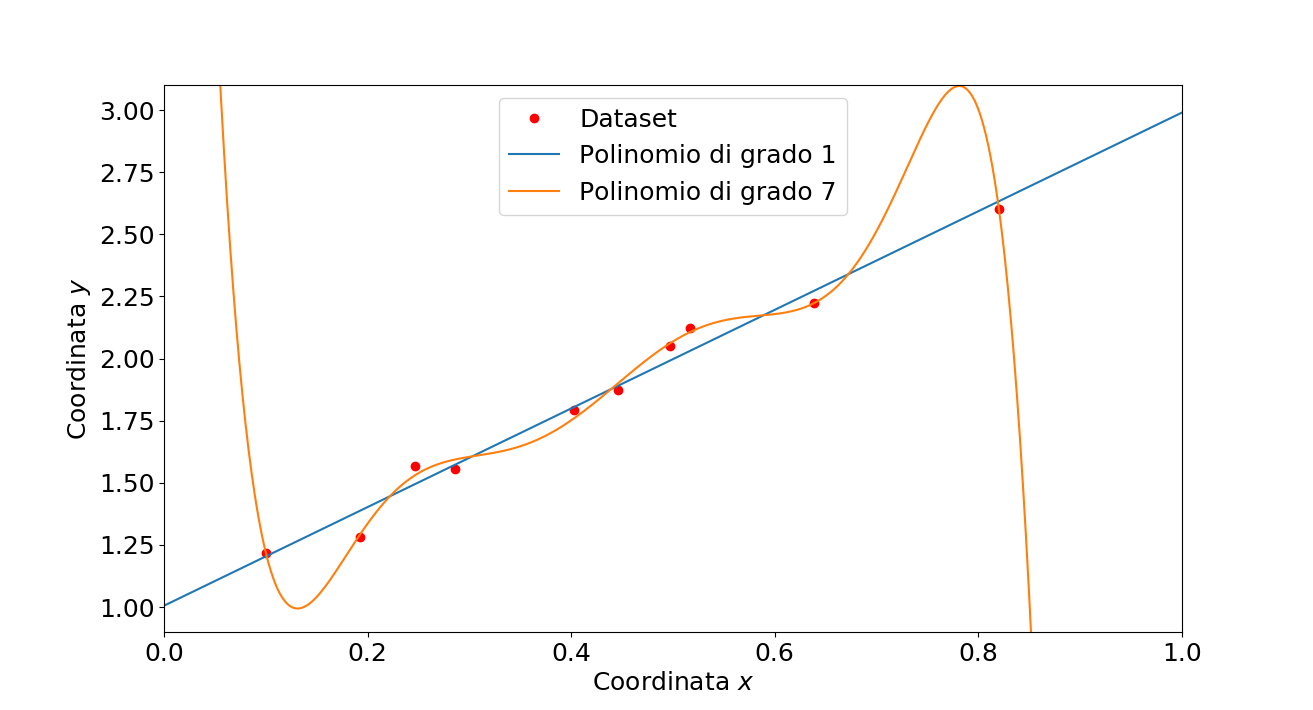
\includegraphics[scale=0.5]{chapter_1_overfitting_example}
\caption{\textit{In questo esempio, stiamo cercando di trovare un polinomio che meglio approssima i punti del dataset. Il polinomio di grado 7, pur rappresentando esattamente i punti del dataset non ha capacità di generalizzazione, quindi nella pratica si tenderà ad utilizzare il polinomio di grado 1.}}
\label{fig:ch_1_overfitting}
\end{figure}

Questa tecnica è detta \textit{regolarizzazione} (o \textit{regularization}) e implica l'aggiunta di un \textit{termine di 
regolarizzazione} $R(\bm{\beta})$ alla \textit{loss function}. Nel caso dei regressori lineari il \textit{termine di 
regolarizzazione} imporrà una penalità sul vettore dei pesi che deve essere stimato.
\begin{equation}
\min_{\bm{\beta}} \sum_{i=1}^{n} (\bm{x}_i\bm{\beta} - y_i)^2 - \lambda R(\bm{\beta})
\end{equation}
Il termine $\lambda$ controlla l'importanza della regolarizzazione.
\bigskip

La tecnica utilizzata in entrambi i modelli utilizzati in questo lavoro viene chiamata $\textit{LASSO}$, acronimo per 
\textit{Least Absolute Shrinkage and Selection Operator}. Essa serve a ridurre l'\textit{overfitting} e ad applicare 
una selezione sulle varie feature disponibili. Infatti, un modello regolarizzato con LASSO tenderà ad assegnare un peso 
positivo a poche feature, determinando così quali sono i regressori che contribuiscono in modo maggiore. Inoltre, la 
regolarizzazione LASSO è indicato nei casi di multicollinerità, cioè quando due o più feature sono altamente correlate tra di 
loro (LASSO ne sceglie solo una ed evita di includere nel modello finale le altre, visto che non diminuirebbero l'entropia 
del modello). Nel caso di \textit{LASSO}, il \textit{termine di regolarizzazione} corrisponde alla norma 1, cioè 
$R(\bm{\beta}) = \norm{\bf{\beta}}_1 = \sum_{i=0}^k \beta_i$. 
In questo caso, le due \textit{loss function} \eqref{eq:GLM_minimize} e 
\eqref{eq:GLM_minimize} vengono ridefinite come:
\begin{gather}
\min_{\bm{\beta}} \sum_{i=1}^{n} (\bm{x}_i\bm{\beta} - y_i)^2 + \lambda\norm{\bm{\beta}}_1 \label{eq:OLS_LASSO} \\
\min_{\bm{\beta}} -\sum_{i=1}^n (y_i\theta x_i - e^{\theta x_i} )  + \lambda\norm{\bm{\beta}}_1 \label{eq:GLM_LASSO}
\end{gather}  

Per stimare il parametro $\lambda$ abbiamo utilizzato la tecnica di \textit{cross-validation}. Essa consiste nel suddividere il 
dataset in $k$ partizioni di uguale numerosità, $k-1$ verrano utilizzate per il \textit{training} mentre l'unica rimanente 
verrà utilizzata per il \textit{testing}. La procedura viene poi ripetuta $k$ volte in modo che ogni partizione abbia sia 
stata utilizzata come \textit{testing set}. Attraverso l'utilizzo di questo metodo possiamo avere maggiori informazioni su 
come il modello finale si comporterà con dati nuovi (cioè quanto il modello è capace di generalizzare). Inoltre, questo 
metodo permette appunto di stimare certi parametri del modello, in modo che il loro valore massimizzi le performance 
dell'algoritmo (o minimizzino al meglio la \textit{loss function}).   

\section{Implementazione}
\bigskip

Per la realizzazione del codice, sono stati utilizzati due framework in Python che possiedono l'implementazione dei metodi
sopracitati. La suite \textit{scikit-learn} \cite{scikit-learn} ha fornito il modello lineare semplice, regolarizzato con 
\textit{LASSO} e validato attraverso \textit{cross-validation}, chiamato \textit{LassoCV}. Per il modello lineare 
generalizzato di Poisson è stato usato il framework \textit{glmnet} \cite{GLMNET} che ha fornito il metodo \textit{cvglmnet} 
(anch'esso con \textit{LASSO}+\textit{cross-validation}). Entrambe le librerie utilizzate minimizzano funzioni che sono 
leggermente diverse da quelle presentate precedentemente (in particolare \eqref{eq:OLS_LASSO} e \eqref{eq:GLM_LASSO}), che 
però sono essenzialmente equivalenti ai fini dell'esperimento vero e proprio. 
\begin{gather}
	\min_{\bm{\beta}} \frac{1}{2n}\sum_{i=1}^n \norm{\bm{\beta} x_i -y_i}_{2}^2 + \lambda\norm{\bm{\beta}}_1 	\qquad
	\min_{\bm{\beta}} -\frac{1}{n}\sum_{i=1}^n (y_i\bm{\beta} x_i - e^{\bm{\beta} x_i} ) + \lambda\norm{\bm{\beta}}_1
\end{gather}

\newpage